\section{Global Statistics}
According to \cite{jemal2011global}, lung cancer is one of the most commonly diagnosed cancers worldwide and remains a leading cause of cancer-related deaths. According to the latest estimates by the \textbf{World Health Organization (WHO)} and the \textbf{Global Cancer Observatory (GLOBOCAN)}:
\begin{itemize}
    \item Lung cancer accounted for approximately \textbf{2.2 million new cases} and over \textbf{1.8 million deaths} globally in 2020.
    \item It represents about \textbf{11.4\% of all new cancer cases} and \textbf{18\% of all cancer deaths}, making it the most fatal cancer globally.
    \item The incidence rate is significantly higher in \textbf{men}, with nearly \textbf{1.4 million cases}, compared to approximately \textbf{770,000 cases in women}.
\end{itemize}

Geographically, the highest incidence rates are observed in:
\begin{itemize}
    \item \textbf{Eastern Europe} and \textbf{Eastern Asia}: High smoking prevalence drives these rates.
    \item \textbf{North America} and \textbf{Western Europe}: Advanced diagnostics contribute to the detection of cases, including early stages.
\end{itemize}
\begin{figure}[h!]
    \centering
    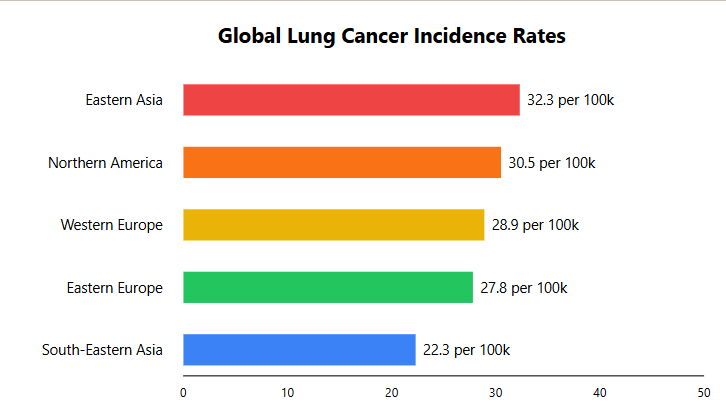
\includegraphics[width=0.8\textwidth]{images/lunc cancer global.png}
    \caption{Charts illustrating global lung cancer statistics}
    \label{fig:lung_stats}
\end{figure}
\newpage
\section{Lung Cancer in India}
Lung cancer is a significant public health challenge in India, with the following key statistics, according to \cite{singh2021lung}:
\begin{itemize}
    \item \textbf{Incidence:} Lung cancer ranks among the \textbf{top three cancers in men} and is increasingly common in women. In 2020, there were approximately \textbf{72,000 new cases} of lung cancer in India.
    \item \textbf{Mortality:} Lung cancer accounted for nearly \textbf{66,000 deaths}, making it a leading cause of cancer-related fatalities in the country.
    \item \textbf{Trends:} While smoking remains the primary cause, rising pollution levels, exposure to industrial carcinogens, and passive smoking are contributing factors. Non-smokers constitute a growing proportion of cases, especially among women.
\end{itemize}
\begin{figure}[h!]
    \centering
    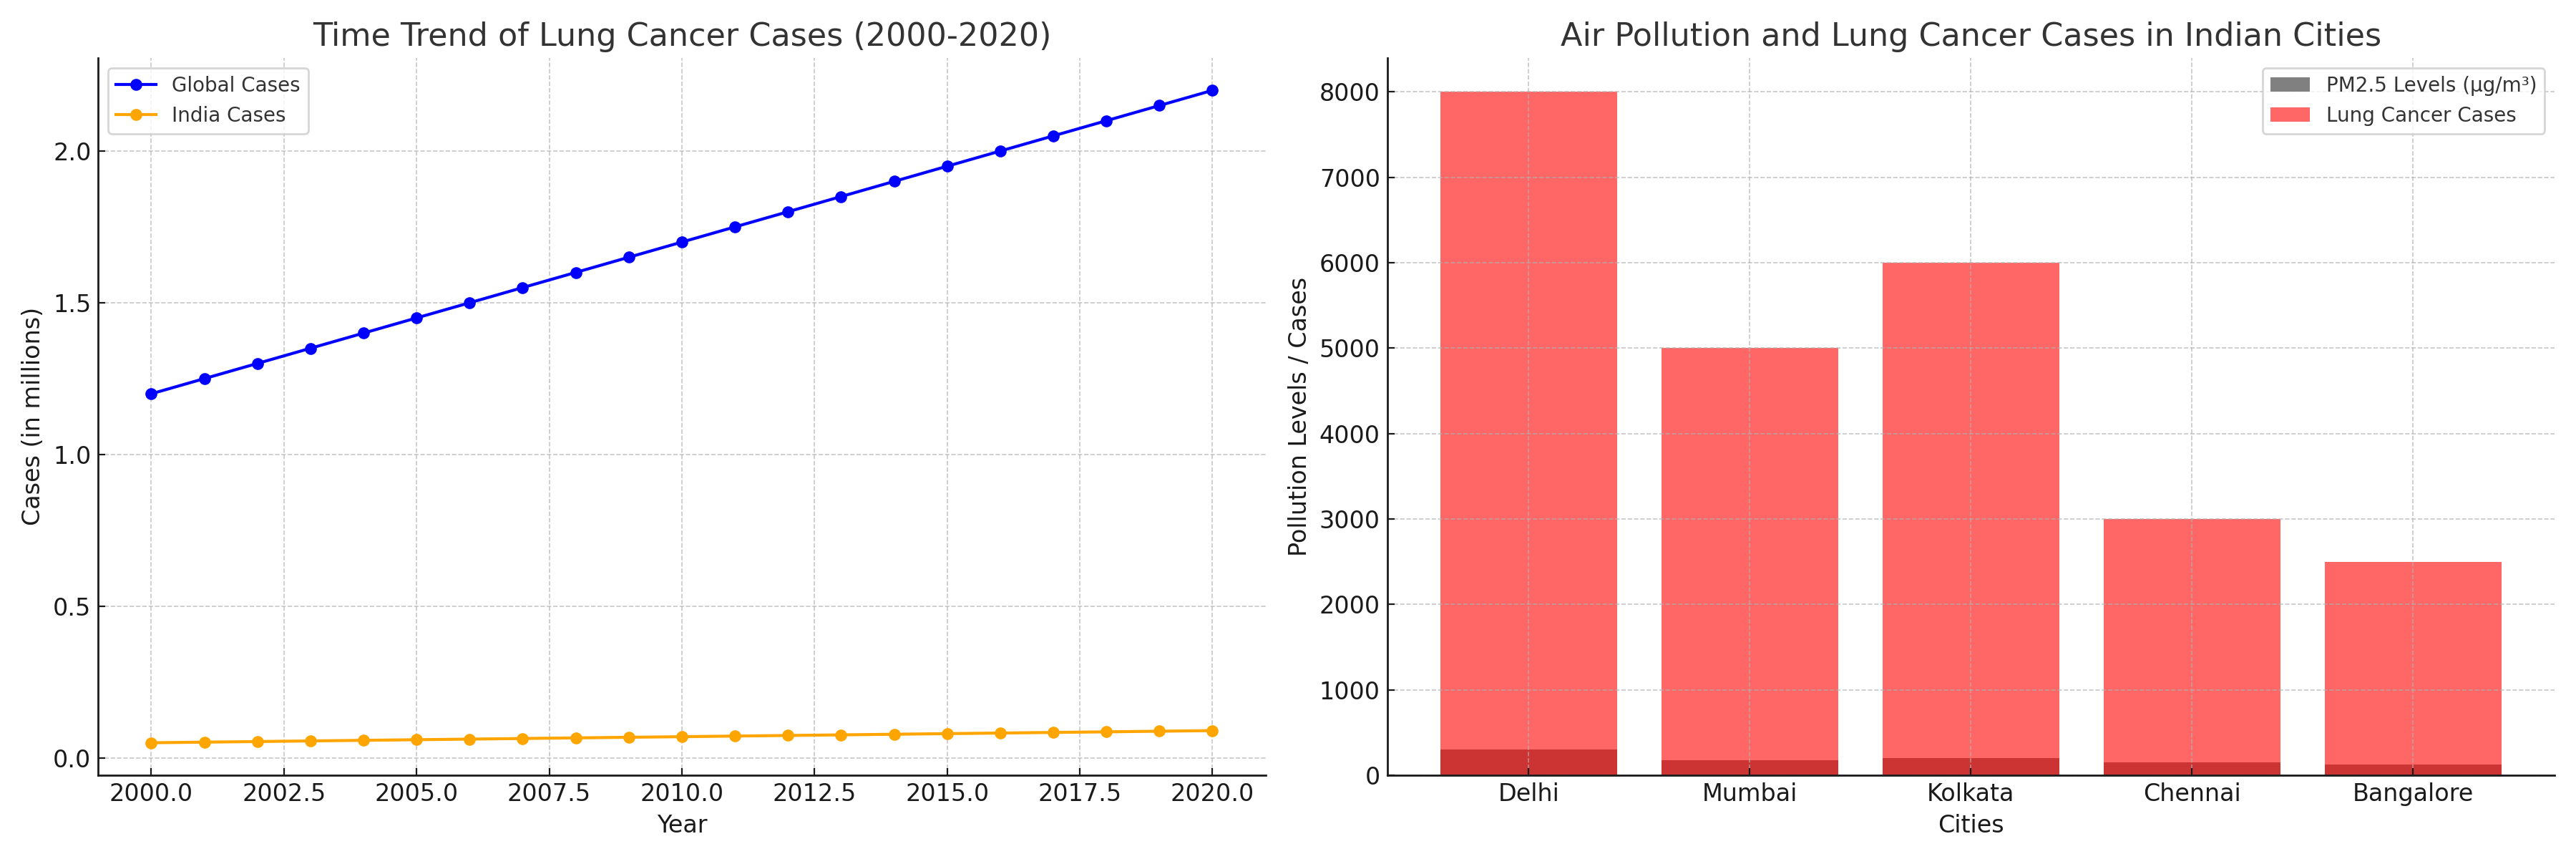
\includegraphics[width=\textwidth]{images/lung_cancer_additional_charts.png}
    \caption{Charts illustrating global and Indian lung cancer statistics}
    \label{fig:lung_stats_2}
\end{figure}
\section{Gender Distribution of Lung Cancer in India}

Lung cancer incidence in India shows significant variation between genders. Key observations are outlined below:

\subsection{Incidence Among Men and Women}

According to the study published in \cite{meza2015lung}
\begin{itemize}
    \item \textbf{Men:} Lung cancer remains one of the leading cancers among men, accounting for approximately \textbf{70-75\% of total cases}. This high prevalence is primarily attributed to smoking (bidi and cigarette use), occupational exposure to carcinogens, and outdoor air pollution.
    \item \textbf{Women:} Though less common, lung cancer cases among women are increasing due to factors like \textbf{indoor air pollution} from biomass fuel, passive smoking, and exposure to environmental pollutants. Non-smoking-related cases constitute a significant proportion.
\end{itemize}

\subsection{Risk Factors in Gender Distribution}
In accordance to the study published in \cite{huang2022distribution}
\begin{itemize}

    \item \textbf{Men:} Smoking remains the dominant factor, contributing to the majority of cases. Occupational hazards and outdoor air pollution also play significant roles.
    \item \textbf{Women:} A large proportion of women diagnosed with lung cancer are \textbf{non-smokers}. Indoor air pollution and passive smoking are major contributors.
\end{itemize}

\subsection{Trends Over Time}
According to \cite{jemal2001recent}:
\begin{itemize}

    \item A \textbf{decline in smoking rates among men} has contributed to a slower increase in lung cancer cases in this group.
    \item An \textbf{increase in non-smoking-related cases among women} is evident, largely due to environmental and lifestyle changes.
\end{itemize}

\begin{figure}[h!]
    \centering
    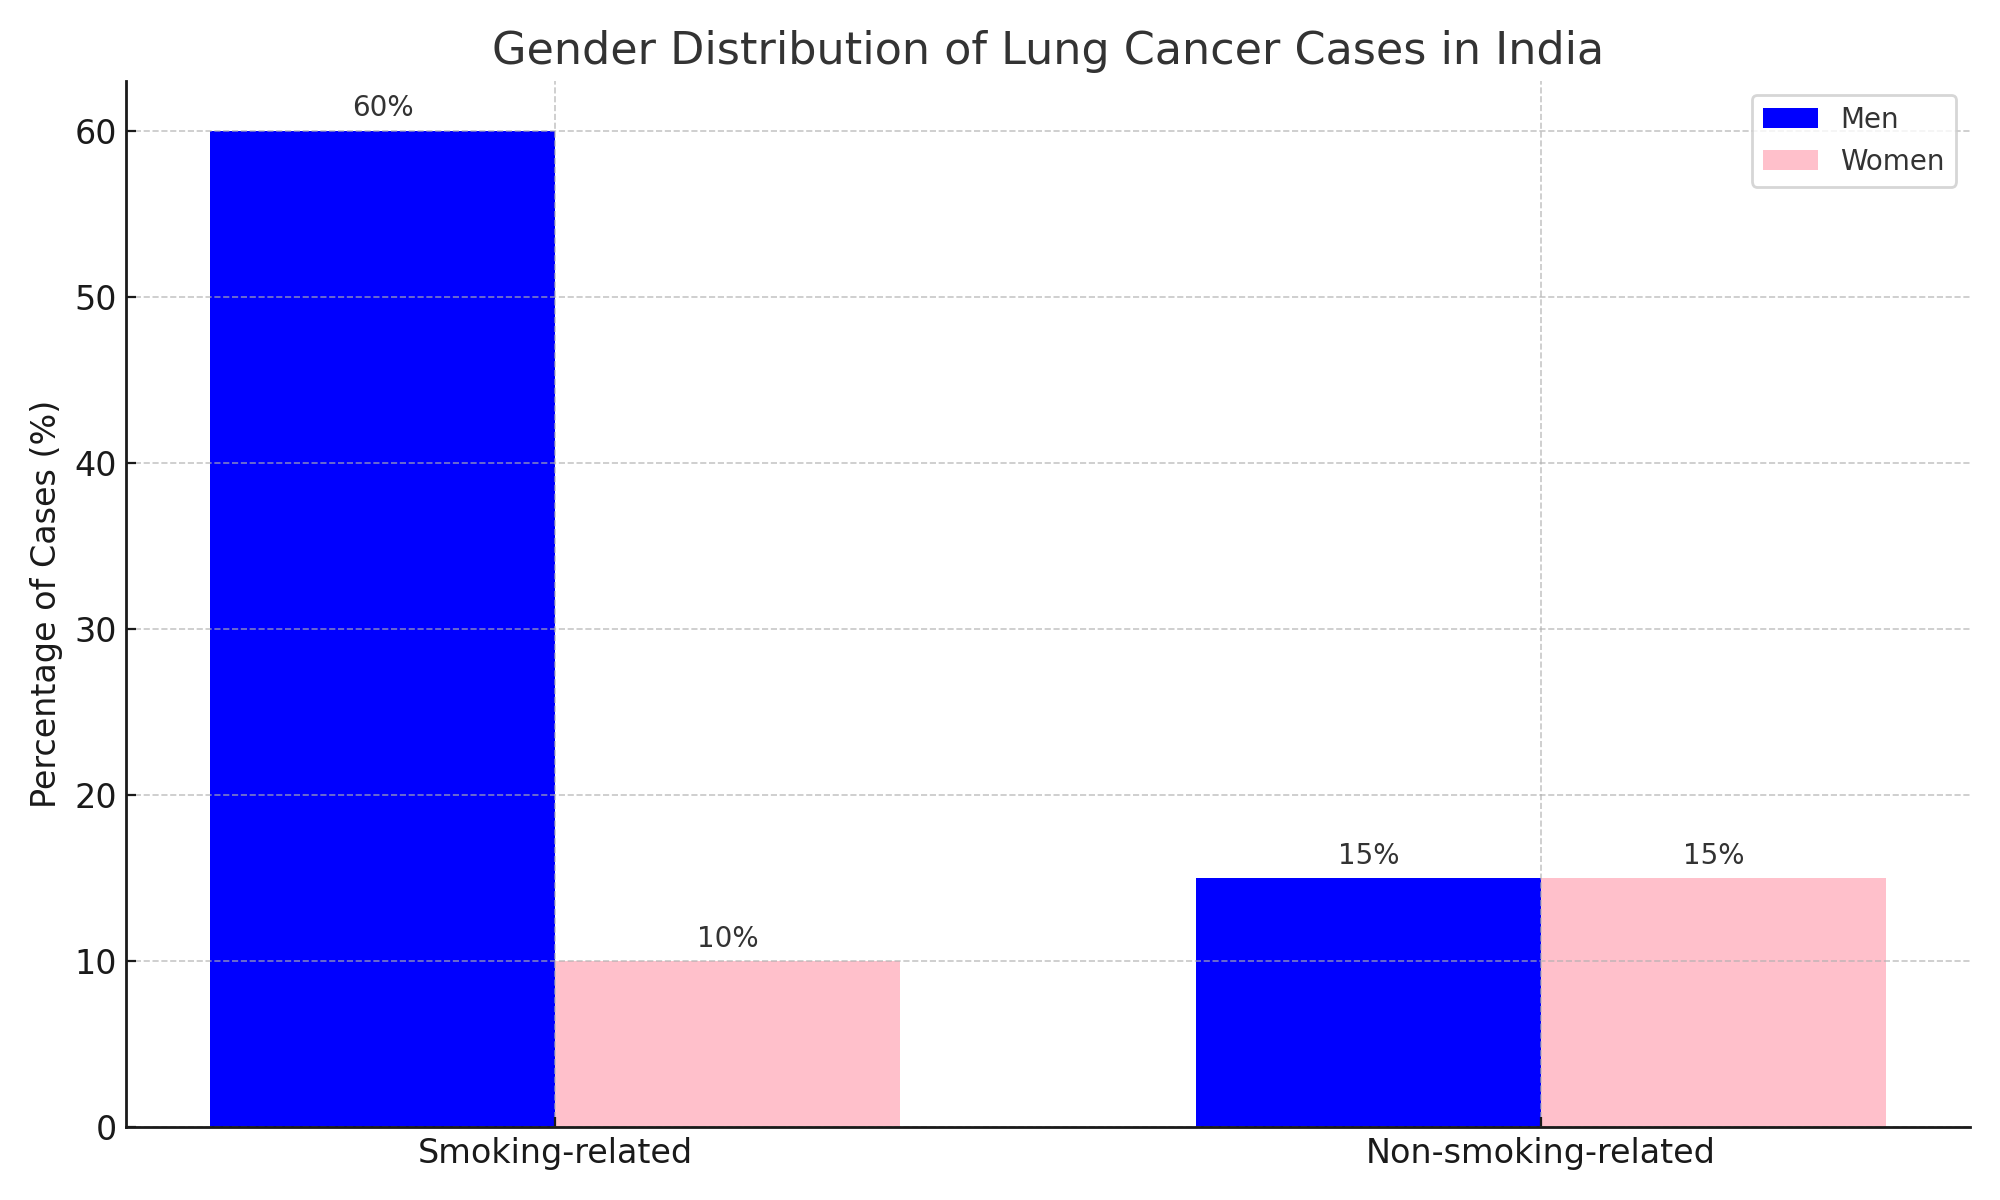
\includegraphics[width=0.8\textwidth]{images/lung_cancer_gender_distribution_chart.png}
    \caption{Gender distribution of lung cancer cases in India}
    \label{fig:gender_distribution}
\end{figure}

\section{Risk Factors Contributing to the Statistics}
\begin{enumerate}
    \item \textbf{Smoking:}
    \begin{itemize}
        \item Globally, over \textbf{80\% of lung cancer cases} are attributed to smoking. In India, a large proportion of men smoke tobacco, while \textbf{bidi smoking} and \textbf{chewing tobacco} further exacerbate the risk.
    \end{itemize}
    \item \textbf{Air Pollution:}
    \begin{itemize}
        \item India faces some of the world's worst air quality, with particulate matter (PM2.5) exposure significantly increasing lung cancer risks, particularly in urban areas like Delhi and Mumbai.
    \end{itemize}
    \item \textbf{Occupational Hazards:}
    \begin{itemize}
        \item Prolonged exposure to asbestos, arsenic, and other carcinogens in industrial settings has raised lung cancer incidence in India.
    \end{itemize}
\end{enumerate}

As stated in the study performed in \cite{akhtar2017risk}.

\section{Global and National Efforts}
To combat lung cancer, global initiatives focus on smoking cessation, air quality improvement, and early diagnosis. In India, according to \cite{leiter2023global}:
\begin{itemize}
    \item The \textbf{National Program for Prevention and Control of Cancer, Diabetes, Cardiovascular Diseases, and Stroke (NPCDCS)} supports early screening and treatment.
    \item Anti-tobacco campaigns and regulations have contributed to reducing smoking prevalence.
    \item Awareness programs targeting pollution and occupational safety are gaining momentum.
\end{itemize}

\section{The Path Forward}
Despite advancements, the burden of lung cancer remains high. Efforts to curb smoking, mitigate pollution, and improve healthcare access are critical to addressing the challenges globally and in India. Comprehensive data collection and research will also help shape effective policies and interventions.